\documentclass[border=10pt,multi,tikz]{standalone}
\usepackage{tikz}
\usetikzlibrary{mindmap}
\pagestyle{empty}
%\tikzset{every node/.append style={scale=-0.4}}
\begin{document}
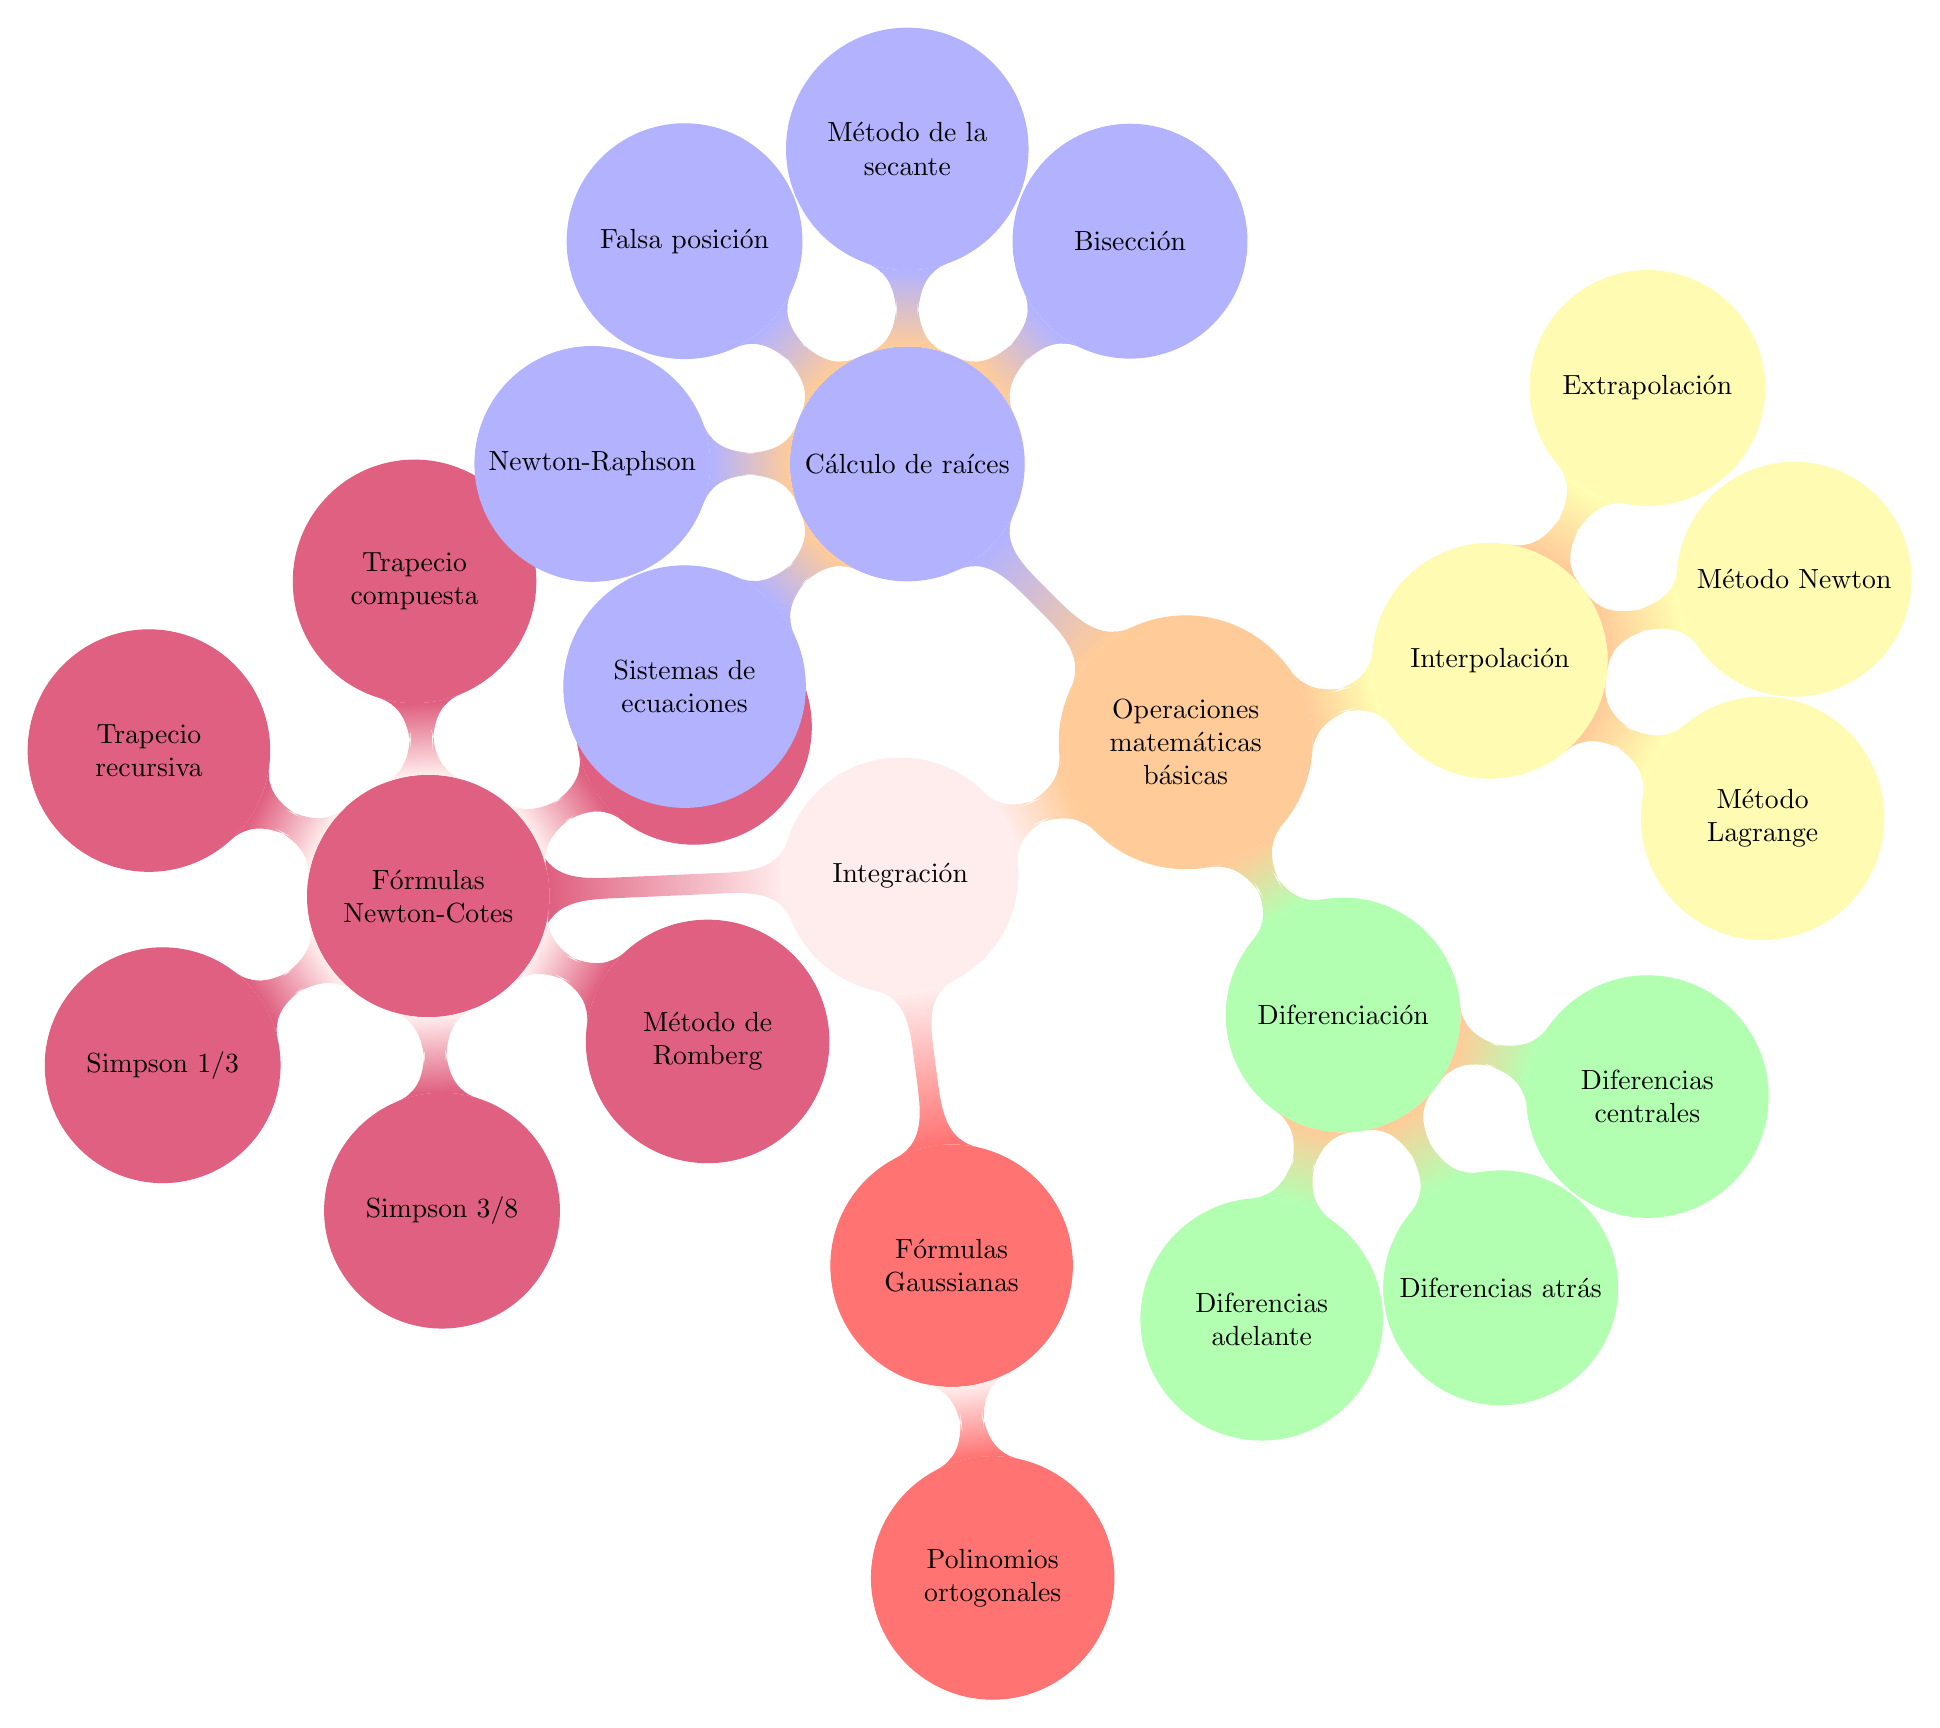
\begin{tikzpicture}[grow cyclic, text width=2.7cm, align=flush center, every node/.style=concept, concept color=orange!40,
    level 1/.style={level distance=4cm,sibling angle=90},
    level 2/.style={level distance=4cm,sibling angle=45},
    level 3/.style={level distance=4cm,sibling angle=60}]
    \node{Operaciones matemáticas básicas}
    child[concept color=pink!30, rotate=-20] { node {Integración} 
        child[concept color=pink!50!purple, level distance= 6cm] { node {Fórmulas Newton-Cotes}
            child { node {Trapecio}}
            child { node {Trapecio compuesta}}
            child { node {Trapecio recursiva}}
            child { node {Simpson $1/3$}}
            child { node {Simpson $3/8$}}
            child { node {Método de Romberg}}
        }
        child[concept color=pink!60!red, rotate=50, level distance= 5cm] { node {Fórmulas Gaussianas}
            child { node {Polinomios ortogonales}}
        }
    }
    child[concept color=green!30, rotate=-15] { node {Diferenciación}
        child { node {Diferencias adelante}}
        child { node {Diferencias atrás}}
        child { node {Diferencias centrales}}
    }
    child[concept color=yellow!30, rotate=-30] { node {Interpolación}
        child { node {Método \\ Lagrange}}
        child { node {Método Newton}}
        child { node {Extrapolación}}
    }
    child[concept color=blue!30, level distance=5cm] { node {Cálculo de raíces}
        child { node {Bisección}}
        child { node {Método de la secante}}
        child { node {Falsa posición}}
        child { node {Newton-Raphson}}
        child { node {Sistemas de ecuaciones}}
    };
\end{tikzpicture}
\end{document}